\chapter{Case Studies of Argument}
\label{case}
This chapter consists of gathering social media data from three ``live'' sources from the web and annotating them with a categorisation system based on the categories reviewed in Chapter \ref{expert}. The distribution of social features (such as replies etc.) and annotations is examined and discussed, and a narrative analysis of three threads is conducted, to discuss some of the features that can be observed on different social platforms in different contexts.

\section{Methodology}

\subsection{Data Sample}
\label{case:method:sample}
Social media posts for this experiment were sourced from Facebook, Twitter and Reddit. From Facebook and Twitter, posts were collected by gathering the 100 most recent posts from five major news distribution networks (\textit{BBC News}, \textit{Sky News}, \textit{CNN News}, \textit{The Guardian}, and \textit{The Daily Mail}) and all replies associated with them. Because of the ``subreddit'' structure of Reddit (there are many ``sub'' sites focusing on individual topics), and becuase these institutions do not maintain official accounts or an otherwise high-profile, active presence on Reddit, this potion of the data sample was sourced instead by collecting the top 500 ``hot'' posts from the World News subreddit\footnote{https://www.reddit.com/r/worldnews/}). ''Hot'' posts, the default view of subreddits, are determined by those with the most upvotes, and are weighted towards more recently active posts \citep{van2011human}.

These threads were then pruned to ensure they contained some form of discourse; that is to say they contained at least two replies, made by at least two different users. Applying this filter resulted in 500 threads from Facebook, 403 from Twitter and 247 from Reddit.

These threads were then examined based on a number of different factors to determine the shape of a ``typical'' thread for each platform. These factors were the \textit{total comments}, \textit{comment length}, \textit{comments per user} and \textit{replies}. Tables \ref{table:case:number_comment}, \ref{table:case:comment_length}, \ref{table:case:comments_per_user}, and \ref{table:case:replies} show a further breakdown of each of the measures used to determine a typical thread for this purpose. These graphs are also shown in Appendix \ref{socialgraphs}.

Table \ref{table:case:number_comment} (and Graphs \ref{socialgraphs:comments:facebook}, \ref{socialgraphs:comments:twitter} and \ref{socialgraphs:comments:reddit}) shows the distribution of the total number of comments in each thread. Naturally, the minimum number of comments for each thread is three; the original post, and two additional, the qualify it as discursive. However, the maximum number of comments was substantially larger, and varied hugely between platforms. Twitter had the smallest range, with 193, and a correspondingly tighter spread. Both Facebook and Reddit had a much greater maximum, with approximately 2500 and 4000 respectively. However, in both cases, these were decidedly outliers. 

Table \ref{table:case:comment_length} (and Graphs \ref{socialgraphs:length:facebook}, \ref{socialgraphs:length:twitter} and \ref{socialgraphs:length:reddit}) shows the distribution of the average comment length in each thread. In a similar pattern to the total number of comments, the length of comments on Facebook and Reddit also displays a  distribution of a curve centred around the lower end of the range with a `long tail' of outliers. The distribution of comment lengths for Twitter appears as a more traditional bell-curve. This is likely due to the upper-limit on comment length, restricting the total size of comments that users can post.

Table \ref{table:case:comments_per_user} (and Graphs \ref{socialgraphs:user:facebook}, \ref{socialgraphs:user:twitter} and \ref{socialgraphs:user:reddit}) shows the distribution of the total number of comments made by each user, in each thread. All three platforms had a very low number of different comments per user, Facebook in particular never exceeding 1. Twitter and Reddit both had mean and median values close to 1, with $\sigma < 0.7$ and $\sigma < 0.5$ respectively.

Table \ref{table:case:replies} (and Graphs \ref{socialgraphs:replies:facebook}, \ref{socialgraphs:replies:twitter} and \ref{socialgraphs:replies:reddit}) shows the distribution of the total number of direct replies to other comments within each thread. Interestingly, Facebook appeared to have zero direct intra-thread replies. Whether this is due to people unwilling to use the (at the time) new feature, or due to already having other methods (such as tagging) to denote replies is not known.


Threads that fell outside of the interquartile range were removed from the sample. This left 139 Facebook threads (with a total of 14,556 individual posts), 113 Twitter threads (with a total of 1,021 individual posts), and 52 Reddit threads (with a total of 1,123 individual posts.

\begin{table}
\centering
\caption{Distribution of total number of comments in each thread}
\label{table:case:number_comment}
\begin{tabular}{ !p{3cm} | ^r ^r ^r ^r ^r ^r ^r}
\rowstyle{\bfseries} Platform & Min. & \pbox{2cm}{Lower\\ Quartile} & Median & \pbox{2cm}{Upper\\ Quartile} & Max. & Mean & $\sigma$\\
\hline
Facebook  &  3.00 & 43.00 & 96.00 & 189.00 & 2478.00 & 179.976 & 274.449 \\
Twitter  &  3.00 & 5.00 & 9.00 & 15.00 & 193.00 & 11.717 & 12.693 \\
Reddit  &  3.00 & 4.00 & 10.00 & 70.00 & 4938.00 & 157.081 & 522.048 \\
\end{tabular}
\end{table}


\begin{table}
\centering
\caption{Distribution of comment length (in characters) in each thread}
\label{table:case:comment_length}
\begin{tabular}{ !p{3cm} | ^r ^r ^r ^r ^r ^r ^r}
\rowstyle{\bfseries} Platform & Min. & \pbox{2cm}{Lower\\ Quartile} & Median & \pbox{2cm}{Upper\\ Quartile} & Max. & Mean & $\sigma$\\
\hline
Facebook  &  24.00 & 68.00 & 103.50 & 161.25 & 715.00 & 127.936 & 90.983 \\
Twitter  &  38.00 & 69.00 & 83.00 & 96.00 & 136.00 & 82.553 & 18.835 \\
Reddit  &  27.00 & 97.00 & 173.00 & 260.50 & 697.00 & 200.870 & 132.320 \\
\end{tabular}
\end{table}


\begin{table}
\centering
\caption{Distribution of the number of comments per user in each thread}
\label{table:case:comments_per_user}
\begin{tabular}{ !p{3cm} | ^r ^r ^r ^r ^r ^r ^r}
\rowstyle{\bfseries} Platform & Min. & \pbox{2cm}{Lower\\ Quartile} & Median & \pbox{2cm}{Upper\\ Quartile} & Max. & Mean & $\sigma$\\
\hline
Facebook  &  1.00 & 1.00 & 1.00 & 1.00 & 1.00 & 1.000 & 0.000 \\
Twitter  &  1.00 & 1.00 & 1.00 & 1.00 & 13.00 & 1.062 & 0.637 \\
Reddit  &  1.00 & 1.00 & 1.00 & 1.00 & 4.00 & 1.182 & 0.480 \\
\end{tabular}
\end{table}


\begin{table}
\centering
\caption{Distribution of the number of internal replies in each thread}
\label{table:case:replies}
\begin{tabular}{ !p{3cm} | ^r ^r ^r ^r ^r ^r ^r}
\rowstyle{\bfseries} Platform & Min. & \pbox{2cm}{Lower\\ Quartile} & Median & \pbox{2cm}{Upper\\ Quartile} & Max. & Mean & $\sigma$\\
\hline
Facebook  &  0.00 & 0.00 & 0.00 & 0.00 & 0.00 & 0.000 & 0.000 \\
Twitter  &  1.00 & 4.00 & 7.00 & 14.00 & 192.00 & 10.442 & 12.627 \\
Reddit  &  0.00 & 1.00 & 5.00 & 49.00 & 4372.00 & 129.526 & 443.849 \\
\end{tabular}
\end{table}

\subsection{Annotation}

A classification system was devised based on the previous extensions proposed to the expert review in Chapter \ref{expert}. For this, only the nodes determined present in each locution were required to be marked; as such, no relationships between nodes were taken into account for this data set. The possible categories were as follows: Information, Transition, Logical Attack, Logical Support, Rhetorical Attack, Rhetorical Support, Preference, Entity, Group, Audience, Implied Relationship, and Implied Belief .

These are broadly similar as those proposed to the experts in Chapter \ref{expert}; however, Personal Support/Attack has been explicitly renamed to Rhetorical Support Attack, to encompass instances where it is not a person that is directly being supported or attacked. Similarly, Persona has been renamed Entity, and Faction renamed to Group. Implications were split into two types: Implied Relationship and Implied Belief

During the annotation process, it was deemed necessary to introduce three other categories to account for circumstances not otherwise covered. These categories are as follows: Spam/Advertisement, which encompasses (often automated) posts that promote a business or service unrelated to the discussion; Unknown, which encompasses posts in a language unknown to the annotator, broken or corrupted text or emojis, or any other circumstances in which the intent of the post cannot be reasonably assumed; and None, encompassing circumstances when a post is totally blank, or blank apart from ``tagging'' a user (to alert them of the thread).

%\subsubsection{Intra Rater reliability}

\section{Data Analysis}
\TODO{Move comment length etc. here?}

\TODO{Annotations}
In terms of annotation

Table \ref{table:case:annotations} shows the total number of annotations 

Table \ref{table:case:other_annotations} shows the number of annotations present alongside $n$ other annotations. For example

Table \ref{table:case:combination_annotations} shows how this is 

\begin{table}
\centering
\caption{Classifications present alongside $n$ other classifications}
\label{table:case:annotations}
\begin{tabular}{ l | r }
\textbf{Classification} & \textbf{Total}  \\
\hline
Information & 675 \\
Transition & 71 \\
Logical Attack & 168 \\
Logical Support & 32 \\
Rhetorical Attack &  474\\
Rhetorical Support & 295 \\
Preference & 5 \\
Entity & 534 \\
Group & 89 \\
Audience & 157 \\
Implied Relationship & 7 \\
Implied Belief & 38 \\
Spam/Advertisement & 24 \\
Unknown & 37 \\
None & 42 \\
\textbf{Total} & \\
\end{tabular}
\end{table}


\begin{table}
\centering
\caption{Classifications present alongside $n$ other classifications}
\label{table:case:other_annotations}
\begin{tabular}{ l | r | r | r | r | r | r | r }
\textbf{Classification} & \multicolumn{7}{c}{\pbox{5cm}{\textbf{Number of Other}\\\textbf{ Classifications Present}}}\\
& \textbf{0} & \textbf{1} & \textbf{2} & \textbf{3} & \textbf{4} & \textbf{5} & \textbf{6} \\  
\hline
Information & 216 & 183 & 169 & 64 & 34 & 6 & 3 \\
Transition & 22 & 30 & 10 & 2 & 4 & 3 & 0 \\
Logical Attack & 2 & 112 & 18 & 31 & 3 & 1 & 1 \\
Logical Support & 0 & 24 & 4 & 3 & 0 & 1 & 0 \\
Rhetorical Attack & 48 & 172 & 142 & 65 & 36 & 8 & 3 \\
Rhetorical Support & 30 & 74 & 33 & 84 & 62 & 9 & 3 \\
Preference & 0 & 2 & 2 & 1 & 0 & 0 & 0 \\
Entity & 0 & 196 & 133 & 131 & 62 & 9 & 3 \\
Group & 0 & 15 & 34 & 26 & 10 & 2 & 2 \\
Audience & 0 & 0 & 11 & 80 & 56 & 7 & 3 \\
Implied Relationship & 0 & 0 & 2 & 5 & 0 & 0 & 0 \\
Implied Belief & 0 & 1 & 15 & 17 & 4 & 1 & 0 \\
Spam/Advertisement & 23 & 1 & 0 & 0 & 0 & 0 & 0 \\
Unknown & 37 & 0 & 0 & 0 & 0 & 0 & 0 \\
None & 42 & 0 & 0 & 0 & 0 & 0 & 0 \\
\end{tabular}
\end{table}


\begin{sidewaystable}
\centering
\caption{Posts that are classified as (at least) both $x$ and $y$}
\label{table:case:combination_annotations}
\begin{tabular} { l  | r | r | r | r | r | r | r | r }
 & \textbf{Information} & \textbf{Transition} & \pbox{3cm}{\textbf{Logical} \\ \textbf{Attack}} & \pbox{3cm}{\textbf{Logical} \\ \textbf{Support}} & \pbox{3cm}{\textbf{Rhetorical} \\ \textbf{Attack}} & \pbox{3cm}{\textbf{Rhetorical} \\ \textbf{Support}} & \textbf{Preference} & \textbf{Entity} \\
\hline
Information  &  N/A  &  25  &  159  &  31  &  217  &  90  &  4  &  215 \\
Transition  &  25  &  N/A  &  9  &  0  &  15  &  7  &  0  &  14  \\
Logical Attack  &  159  &  9  &  N/A  &  4  &  43  &  7  &  1  &  34  \\
Logical Support  &  31  &  0  &  4  &  N/A  &  5  &  3  &  0  &  6   \\
Rhetorical Attack  &  217  &  15  &  43  &  5  &  N/A  &  61  &  2  &  330 \\
Rhetorical Support  &  90  &  7  &  7  &  3  &  61  &  N/A  &  0  &  249 \\
Preference  &  4  &  0  &  1  &  0  &  2  &  0  &  N/A&  1   \\
Entity  &  215  &  14  &  34  &  6  &  330  &  249  &  1  &  N/A \\
Group  &  66  &  1  &  9  &  2  &  80  &  19  &  1  &  29  \\
Audience  &  42  &  8  &  2  &  1  &  52  &  138  &  0  &  145 \\
Implied Relationship  &  5  &  0  &  0  &  0  &  3  &  2  &  0  &  4   \\
Implied Belief  &  22  &  2  &  1  &  0  &  22  &  4  &  0  &  16  \\
Spam/Advertisement  &  1  &  0  &  0  &  0  &  0  &  0  &  0  &  0   \\
Unknown  &  0  &  0  &  0  &  0  &  0  &  0  &  0  &  0   \\
None  &  0  &  0  &  0  &  0  &  0  &  0  &  0  &  0   \\
\end{tabular}
\begin{tabular} { l  | r | r | r | r | r | r | r  }
 & \textbf{Group} & \textbf{Audience} & \pbox{3cm}{\textbf{Implied} \\ \textbf{Relationship}} & \pbox{3cm}{\textbf{Implied} \\ \textbf{Belief}}  & \textbf{Spam/Advertisement} & \textbf{Unknown} & \textbf{None} \\
\hline
Information &  66  &  42  &  5  &  22  &  1  &  0  &  0 \\
Transition &  1  &  8  &  0  &  2  &  0  &  0  &  0 \\
Logical Attack &  9  &  2  &  0  &  1  &  0  &  0  &  0 \\
Logical Support &  2  &  1  &  0  &  0  &  0  &  0  &  0 \\
Rhetorical Attack  &  80  &  52  &  3  &  22  &  0  &  0  &  0 \\
Rhetorical Support &  19  &  138  &  2  &  4  &  0  &  0  &  0 \\
Preference   &  1  &  0  &  0  &  0  &  0  &  0  &  0 \\
Entity &  29  &  145  &  4  &  16  &  0  &  0  &  0 \\
Group &  N/A  &  7  &  4  &  14  &  0  &  0  &  0 \\
Audience &  7  &  N/A  &  0  &  21  &  0  &  0  &  0 \\
Implied Relationship &  4  &  0  &  N/A  &  1  &  0  &  0  &  0 \\
Implied Belief &  14  &  21  &  1  &  N/A  &  0  &  0  &  0 \\
Spam/Advertisement &  0  &  0  &  0  &  0  &  N/A  &  0  &  0 \\
Unknown &  0  &  0  &  0  &  0  &  0  &  N/A  &  0 \\
None &  0  &  0  &  0  &  0  &  0  &  0  &  N/A \\
\end{tabular}
\end{sidewaystable}



\section{Narrative Account}

\newcommand{\scaleCaseThread}{0.7}
In this section, one thread from each of the social media platforms is examined as a case study. These threads are reproduced in full in Appendix \ref{threads}.

\subsection{Facebook}
Section \ref{threads:facebook} shows a thread on Facebook, starting with the post:

\textit{``US election 2016: Trump wins Nevada - Strengthening his position in the Republican presidential race.''}

The overall structure of this thread is very flat, with no nested replies. The majority of users post a comment sharing their own views, predominantly supporting or attacking Trump. Often, these posts are self-contained, relating to no other information in the thread aside from the original article. These range from relatively short, such as:

\textit{``Say `NO' to Trump Sheeples''}

or:

\textit{``Yes trump love it .from the UK''}

which simply voice support or opposition to Trump as a candidate, and implicitly signal the
user's own political beliefs. In contrast, some users post highly detailed and articulate arguments, explicitly spelling out why they believe a certain way:

\textit{``Interesting times we live in. I'd really like to see Trump and Sanders win their respective party's nomination. I think they might both force our two political parties to reform and produce better candidates. It'd be nice to see them shake up DC too, they're both political outsiders and it seems most establishment politicians aren't very fond of either of them.''}

A number of users post comments simply to tag other users (presumably friends) to notify
them of the story. Some users, possibly bots, also use the thread to advertise t-shirts, or other seemingly unrelated news-stories, likely due to the large user-density of Facebook.
Broadly speaking, due to the lack of explicit intra-thread replies, it appears that users mostly use Facebook to signal their own views, without directly engaging in discussion with other users in the same thread, while at the same time using it to highlight particular posts of interest to friends who may not otherwise see them.

Figure \ref{casegraph:time:facebook} shows that the vast majority of comments made are rhetorical in nature, and the majority of those are attacks. This is ultimately likely to be down to the topic at hand; topics about a particular individual often draw a large about of ire from the social web, particularly one as divisive as a politician. Figure \ref{casegraph:user:facebook} mirrors this, showing that most users post a rhetorical comment. It also highlights that, throughout the entire thread, only one user posts more than once.
 
\begin{figure}
\centering
\includegraphics[scale=\scaleCaseThread]{case threads/time/Facebook.png}
\caption{Cumulative logical and rhetorical tactics over time on Facebook}
\label{casegraph:time:facebook}
\end{figure}

\begin{figure}
\centering
\includegraphics[scale=\scaleCaseThread]{case threads/user/Facebook.png}
\caption{Logical and rhetorical tactics per user on Facebook}
\label{casegraph:user:facebook}
\end{figure}


\subsection{Twitter}
Section \ref{threads:twitter} shows a thread on Twitter, starting with the post:

\textit{``Kesha `in tears' after judge denies her release from Sony where producer allegedly raped her https://t.co/thYQgcH9AW https://t.co/XBnz5x5fIJ''}

Here, more intra-thread replies can be observed, with users directly and explicitly replying to one-another, either to make a counterpoint:

\textit{``@Btwsts @DailyMailCeleb you do realise thats slander without proof, If sony wanted too they could sue you. People have been sued for less.''}

or to request more information on the topic:

\textit{``@Btwsts what rape?''}

(if taken literally; read another way, this post could instead be voicing disbelief/scepticism, again highlighting the difficulties with a lack of tone or other familiar vocal or physical language cues).

One user also reposts the entirety of the original post, verbatim:

\textit{``RT @DailyMailCeleb: Kesha 'in tears' after judge denies her release from Sony where producer allegedly raped her https://t.co/thYQgcH9AW ht…''}

By doing this, they share this content with their own followers as well. However, in doing this they also choose to reply to the original post, which is not required.

\TODO{The twitter graphs don't seem quite right; not enough posts? Check those numbers}

\begin{figure}
\centering
\includegraphics[scale=\scaleCaseThread]{case threads/time/Twitter.png}
\caption{Cumulative logical and rhetorical tactics over time on Twitter}
\label{casegraph:time:twitter}
\end{figure}

\begin{figure}
\centering
\includegraphics[scale=\scaleCaseThread]{case threads/user/Twitter.png}
\caption{Logical and rhetorical tactics per user on Twitter}
\label{casegraph:user:twitter}
\end{figure}


\subsection{Reddit}
Section \ref{threads:reddit} shows a thread on Reddit, starting with the post:
	
\textit{``Brexit against Scotland's wishes would `almost certainly' trigger independence referendum, warns Nicola Sturgeon''}.

This thread had many more internal replies than either of the others, with discussion moving back and forth between different ``sub-threads'': Reddit, unlike the two previously observed platforms highlights replies by indenting them within the body of the page for greater clarity.

Comments routinely refer directly to the comments they reply to, for example:

\textit{``You actually can call for a referendum whenever you want.''}

%\rule{\textwidth}{1pt}

\textit{``Like France, Ireland etc.''}

or in other instances:

\textit{``that arsey dwarf is (one of ) the reasons why we've got a tory government''}

%\rule{\textwidth}{1pt}

\textit{``If every single person in Scotland voted labour, the Tories still would have won''}

%\rule{\textwidth}{1pt}

\textit{``the snp claimed labour would need them to govern, and that scotland would have the sway over a future labour government.}

\textit{great for her home audience, but the tories used it to make labour look like their puppet- a british parliament working for scotland. }

\textit{so scotland gets all those mps but as you say, not enough to decide any policies AND they ensured a tory victory.}

\textit{edited for my shocking spelling''}

This highlights that, on Reddit, people are more inclined to argue or discuss in good-faith, even when resorting to crude humour or vulgar language. This is perhaps unsurprising: as users must specifically browse to this subreddit, rather than come across such posts by chance.

Interestingly, this thread also contains a post from a bot (that acknowledges itself as such) that provides a summary of the article reference in the original post, for users too busy or unwilling to read the entire article, allowing them to still  contribute to the discussion.

Figure \ref{casegraph:time:reddit} shows that while there is still a clear prevalence of attack over support (as might be expected in an argument) although interestingly, in this topic at least, logical attacks are favoured over rhetorical attacks and, within rhetorical tactics, support is favoured over attack. Figure \ref{casegraph:user:reddit} shows that some users choose to post only a single comment, using various tactics, others engage further, posting multiple times and using an array of different tactics, both logical and rhetorical.


\begin{figure}
\centering
\includegraphics[scale=\scaleCaseThread]{case threads/time/Reddit.png}
\caption{Cumulative logical and rhetorical tactics over time on Reddit}
\label{casegraph:time:reddit}
\end{figure}

\begin{figure}
\centering
\includegraphics[scale=\scaleCaseThread]{case threads/user/Reddit.png}
\caption{Logical and rhetorical tactics per user on Reddit}
\label{casegraph:user:reddit}
\end{figure}


\section{Summary}
This chapter examined the structure of ``normal'' social media threads and compared them with one another, as well as a set of individual case-studies.



From the case studies it can be seen, anecdotally at least, that Facebook users tend to post as a way of presenting their opinion to the audience, without necessarily engaging further in the discussion: a ``fire and forget'' approach. Conversely, Reddit users seem more proactive with engaging with the discussion, and other users. This is likely due to the fact that 


